%
% elliptisch.tex
%
% (c) 2021 Prof Dr Andreas Müller, OST Ostshweizer Fachhochschule
%
\section{Elliptische Kurven
\label{buch:section:elliptische-kurven}}
\index{elliptische Kurve}%
\rhead{Elliptische Kurven}
Das Diffie-Hellman-Verfahren basiert auf der Schwierigkeit, in einem 
Körper $\mathbb{F}_p$ die Gleichung $a^x=b$ nach $x$ aufzulösen.
Die Addition in $\mathbb{F}_p$ wird dazu nicht benötigt.
Es reicht, eine Menge mit einer Multiplikation zu haben, fir die
die Gleichung $a^x=b$ schwierig zu lösen ist.
Ein Halbgruppe wäre also durchaus ausreichend.

Ein Kandidat für eine solche Gruppe könnte der Einheitskreis
$S^1=\{z\in\mathbb{C}\;|\; |z|=1\}$ in der komplexen Ebene sein.
Wählt man eine Zahl $g=e^{i\alpha}$, wobei $\alpha$ ein irrationales
Vielfaches von $\pi$ ist, dann sind alle Potenzen $g^n$ für natürliche
Exponenten voneinander verschieden.
Wäre nämlich $g^{n_1}=g^{n_2}$, dann wäre $e^{i\alpha(n_1-n_2)}=1$ und
somit müsste $\alpha=2k\pi/(n_1-n_2)$ sein.
Damit wäre aber $\alpha$ ein rationales Vielfaches von $\pi$, im Widerspruch
zur Voraussetzung.
Die Abbildung $n\mapsto g^n\in S^1$ ist auf den ersten Blick etwa ähnlich
undurchschaubar wie die Abbildung $n\mapsto g^n\in\mathbb{F}_p$.
Es gibt zwar die komplexe Logarithmusfunktion, mit der man $n$ bestimmen
kann, dazu muss man aber den Wert von $g^n$ mit beliebiger Genauigkeit
kennen, denn die Werte von $g^n$ können beliebig nahe beieinander liegen.

Der Einheitskreis ist die Lösungsmenge der Gleichung $x^2+y^2=1$ für
reelle Koordinaten $x$ und $y$,
doch Rundungsunsicherheiten verunmöglichen den Einsatz in einem 
Verfahren ähnlich dem Diffie-Hellman-Verfahren.
Dieses Problem kann gelöst werden, indem für die Variablen Werte
aus einem endlichen Körper verwendet werden.
Gesucht ist also eine Gleichung in zwei Variablen, deren Lösungsmenge
in einem endlichen Körper eine Gruppenstruktur trägt.
Die Lösungsmenge ist eine ``Kurve'' von Punkten mit
\index{Kurve}%
Koordinaten in einem endlichen Körper.

In diesem Abschnitt wird gezeigt, dass sogenannte elliptische Kurven
über endlichen Körpern genau die verlangen Eigenschaften haben.

\subsection{Definition}
Elliptische Kurven sind Lösungen einer Gleichung der Form
\begin{equation}
Y^2+XY=X^3+aX+b
\label{buch:crypto:eqn:ellipticcurve}
\end{equation}
mit Werten von $X$ und $Y$ in einem geeigneten Körper.
Die Koeffizienten $a$ und $b$ müssen so gewählt werden, dass die
Gleichung~\eqref{buch:crypto:eqn:ellipticcurve} genügend viele
Lösungen hat.
Über den komplexen Zahlen hat die Gleichung natürlich für jede Wahl von
$X$ drei Lösungen.
Für einen endlichen Körper können wir dies im allgemeinen nicht erwarten,
aber wenn wir genügend viele Wurzeln zu $\mathbb{F}$ hinzufügen können wir
mindestens erreichen, dass die Lösungsmenge so viele Elemente hat, 
dass ein Versuch, die Gleichung $g^x=b$ mittels Durchprobierens zu
lösen, zum Scheitern verurteilt ist.

\begin{definition}
\label{buch:crypto:def:ellipticcurve}
Die {\em elliptische Kurve} $E_{a,b}(\Bbbk)$ über dem Körper $\Bbbk$ ist 
\index{elliptische Kurve}%
die Menge
\[
E_{a,b}(\Bbbk)
=
\{(X,Y)\in\Bbbk^2\;|\;Y^2+XY=X^3+aX+b\},
\]
für $a,b\in\Bbbk$.
\end{definition}

\subsection{Visualisierung über dem Körper $\mathbb{R}$}
Um die Anschauung zu vereinfachen, werden wir elliptische Kurven über
dem Körper $\mathbb{R}$ visualisieren.
Die daraus gewonnenen geometrischen Einsichten werden wir anschliessend
algebraisch umsetzen.
In den reellen Zahlen kann man die
Gleichung~\eqref{buch:crypto:eqn:ellipticcurve}
noch etwas vereinfachen.
Indem man in \eqref{buch:crypto:eqn:ellipticcurve} 
quadratisch ergänzt, bekommt man
\begin{align}
Y^2 + XY + \frac14X^2 &= X^3+\frac14 X^2 +aX+b
\notag
\\
\Rightarrow\qquad
v^2&=X^3+\frac14X^2+aX+b,
\label{buch:crypto:eqn:ell2}
\end{align}
indem man $v=Y+\frac12X$ setzt.
Man beachte, dass man diese Substition nur machen kann, wenn $\frac12$
definiert ist.
In $\mathbb{R}$ ist dies kein Problem, aber genau über den Körpern
mit Charakteristik $2$, die wir für die Computer-Implementation
bevorzugen, ist dies nicht möglich.
Es geht hier aber nur um die Visualisierung.

Auch die Form \eqref{buch:crypto:eqn:ell2} lässt sich noch etwas 
vereinfachen.
Setzt man $X=u-\frac1{12}$, dann verschwindet nach einiger Rechnung,
die wir hier nicht durchführen wollen, der quadratische Term
auf der rechten Seite.
Die interessierenden Punkte sind Lösungen der einfacheren Gleichung
\begin{equation}
v^2
=
u^3+\biggl(a-\frac{1}{48}\biggr)u + b-\frac{a}{12}+\frac{1}{864}
=
u^3+Au+B.
\label{buch:crypto:ellvereinfacht}
\end{equation}
In dieser Form ist mit $(u,v)$ immer auch $(u,-v)$ eine Lösung,
die Kurve ist symmetrisch bezüglich der $u$-Achse.
Ebenso kann man ablesen, dass nur diejenigen $u$-Werte möglich sind,
für die das kubische Polynom $u^3+Au+B$ auf der rechten Seite von
\eqref{buch:crypto:ellvereinfacht}
nicht negativ ist.

Sind $u_1$, $u_2$ und $u_3$ die Nullstellen des kubischen Polynoms
auf der rechten Seite von~\eqref{buch:crypto:ellvereinfacht}, folgt
\[
v^2
=
(u-u_1)(u-u_2)(u-u_3)
=
u^3
-(u_1+u_2+u_3)u^2
+(u_1u_2+u_1u_3+u_2u_3)u
-
u_1u_2u_3.
\]
Durch Koeffizientenvergleich sieht man, dass $u_1+u_2+u_3=0$ sein muss.
\begin{figure}
\centering
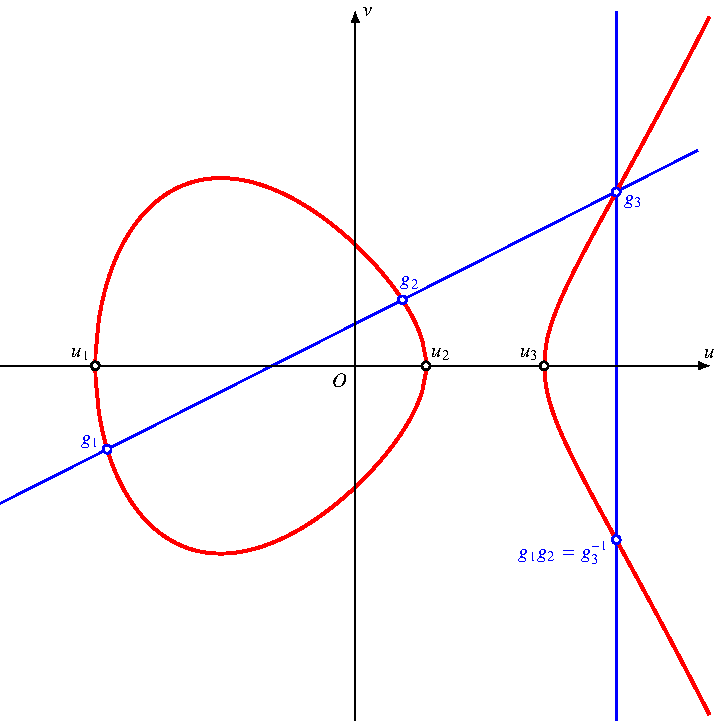
\includegraphics{chapters/90-crypto/images/elliptic.pdf}
\caption{Elliptische Kurve in $\mathbb{R}$ in der Form
$v^2=u^3+Au+B$ mit Nullstellen $u_1$, $u_2$ und $u_3$ des
kubischen Polynoms auf der rechten Seite.
Die blauen Punkte und Geraden illustrieren die Definition der
Gruppenoperation in der elliptischen Kurve.
\label{buch:crypto:fig:elliptischekurve}}
\end{figure}
Abbildung~\ref{buch:crypto:fig:elliptischekurve}
zeigt eine elliptische Kurve in der Ebene $\mathbb{R}^2$.

\subsection{Geometrische Definition der Gruppenoperation}
In der speziellen Form \ref{buch:crypto:ellvereinfacht} ist die
elliptische Kurve symmetrisch unter Spiegelung an der $u$-Achse.
Die Spiegelung ist eine Involution, zweimalige Ausführung führt auf
den ursprünglichen Punkt zurück.
Die Inverse in einer Gruppe hat diese Eigenschaft auch, es ist
daher naheliegend, den gespiegelten Punkt als die Inverse eines
Elementes zu nehmen.

Eine Gerade durch zwei Punkte der
in Abbildung~\ref{buch:crypto:fig:elliptischekurve}
dargestellten Kurve schneidet die Kurve ein drittes Mal.
Die Gruppenoperation wird so definiert, dass drei Punkte der Kurve
auf einer Geraden das Gruppenprodukt $e$ haben.
Da aus $g_1g_2g_3=e$ folgt $g_3=(g_1g_2)^{-1}$ oder
$g_1g_2=g_3^{-1}$, erhält man das Gruppenprodukt zweier Elemente
auf der elliptischen Kurve indem erst den dritten Schnittpunkt
ermittelt und diesen dann an der $u$-Achse spiegelt.

Die geometrische Konstruktion schlägt fehl, wenn $g_1=g_2$ ist.
In diesem Fall kann man die Tangente im Punkt $g_1$ an die Kurve 
verwenden.
Dieser Fall tritt zum Beispiel auch in den drei Punkten 
$(u_1,0)$, $(u_2,0)$ und $(u_3,0)$ ein.

Um das neutrale Element der Gruppe zu finden, können wir 
zwei Punkte $g$ und $g^{-1}$ miteinander verknüpfen.
Die Gerade durch $g$ und $g^{-1}$ schneidet aber die Kurve
kein drittes Mal.
Ausserdem sind alle Geraden durch $g$ und $g^{-1}$ für verschiedene
$g$ parallel.
Das neutrale Element entspricht also einem unendlich weit entfernten Punkt.
Das neutrale Element entsteht immer dann als Produkt, wenn zwei
Punkte die gleiche $u$-Koordinaten haben.

\subsection{Gruppenoperation, algebraische Konstruktion}
Nach den geometrischen Vorarbeiten zur Definition der Gruppenoperation
kann können wir die Konstruktion jetzt algebraisch über einem 
beliebigen Körper umsetzen.

Wir gehen jetzt wieder von der elliptischen Kurve in der Form
\begin{equation}
Y^2+XY=X^3+aX+b
\label{buch:crypto:eqn:grupopgl}
\end{equation}
aus.
Man kann dies auch mit dem Polynom mit zwei Variablen
\[
P(X,Y) = Y^2+XY -X^3-aX-b
\]
schreiben.
Ein Punkt $g=(x,y)$ auf der elliptischen Kurve erfüllt die
Bedingung $P(x,y)=0$.

\subsubsection{Involution}
Zunächst überlegen wir uns wieder eine Involution, welche als Inverse
dienen kann.
Dazu beachten wir, dass die linke Seite der definierenden Gleichung
\eqref{buch:crypto:eqn:grupopgl}
auch als $Y(Y+X)$ geschrieben werden kann.
Die Abbildung $Y\mapsto -X-Y$ macht daraus
\[
(-X-Y)(-X-Y+X)=(X+Y)Y.
\]
Mit dem Punkt $(X,Y)$ ist automatisch auch $(X,-X-Y)$
ein Punkt der elliptischen Kurve.
Dies ist die gesuchte Involution.

\subsubsection{Gerade durch zwei Punkte}
Seien also $g_1=(x_1,y_1)$ und $g_2=(x_2,y_2)$ zwei verschiedene Lösungen
der Gleichung \eqref{buch:crypto:eqn:grupopgl}
Als erstes brauchen wir eine Gleichung für die Gerade durch die beiden
Punkte.
Sei also $l(X,Y)$ eine Linearform derart, dass $l(g_1)=d$ und $l(g_2)=d$
für ein geeignetes $d\in\Bbbk$.
Dann gilt auch für die Punkte
\[
g(t) = tg_1 + (1-t)g_2
\qquad\Rightarrow\qquad
l(g(t))
=
tl(g_1) + (1-t)l(g_2)
=
td+(1-t)d
=
(t+1-t)d
=d.
\]
Jeder Punkt $g$ der Geraden durch $g_1$ und $g_2$ erfüllt einerseits
$l(g)=d$, andererseits lässt er sich in dieser Form schreiben $g(t)$
für ein geeignetes $t\in\Bbbk$ schreiben.

\subsubsection{Dritter Schnittpunkt}
Setzt man jetzt $g(t)$ in die Gleichung~\eqref{buch:crypto:eqn:grupopgl}
ein, erhält man eine kubische
Gleichung in $t$, von der wir bereits zwei Nullstellen kennen, nämlich 
$0$ und $1$.
Die kubische Gleichung muss also durch $t$ und $(t-1)$ teilbar sein.
Diese Berechnung kann man einfach in einem Computeralgebrasystem
durchführen.
Das Polynom ist
\begin{align*}
p(t)
&=
(t-1)^2y_2^2
+
((2t-2t^2) y_1 +(t^2-2t+1)x_2 + (t-t^2)x_1)y_2
+
t^2y_1^2
+
((t-t^2)x_2+t^2 x_1)y_1
\\
&\qquad
+
(t^3-3t^2+3t-1)x_2^3
+
(-3 t^3+6t^2-3t)x_1x_2^2
+
((3t^3-3t^2)x_1^2+at-a)x_2
-
t^3x_1^3
-
atx_1-b
\end{align*}
Da die Punkte $g_1=g(0)$ und $g_2=g(1)$ auf der elliptischen Kurve
liegen, muss das Polynom durch die Nullstellen $t=0$ und $t=1$
haben, es muss also durch $t(t-1)$ teilbar sein.
Teilt man durch $t(t-1)$ bleibt ein Polynom ersten Grades mit
einer einzigen Nullstelle, dem dritten Punkt.
Nach Division durch $t(t-1)$ erhält man als Quotienten
\begin{align}
q(t)
&=
(y_2-y_1)^2 
+
(y_2-y_1) (x_2-x_1)
+
t(x_2-x_1)^3
-
2x_2^3+3x_1x_2^2-x_1^3
\label{buch:ecc:eqn:q(t)}
\end{align}
und den Rest
\begin{align*}
r(t)
&=
t(y_1^2+x_1y_1-x_1^3-ax_1-b)
+
(1-t)(y_2^2+x_2y_2-x_2^3-ax_2-b)
\\
&=
tP(x_1,y_1)
+
(1-t)P(x_2,y_2)
=
0.
\end{align*}
Die Klammerausdrücke verschwinden, da sie gleichbedeutend damit sind,
dass die Punkte Lösungen von \eqref{buch:crypto:eqn:grupopgl} sind.
Dies bestätigt nochmals, dass der Rest $r(t)=0$ ist, dass $p(t)$
also durch $t(1-t)$ teilbar ist.

Für den dritten Punkt auf der Geraden muss $t$ so gewählt werden, dass
$q(t)=0$ ist.
Dies ist aber eine lineare Gleichung mit der Lösung
\begin{align*}
t
&=
-\frac{
(y_1-y_2)^2
+
(y_2-y_1)(x_2-x_1)
-2x_2^3+3x_1x_2^2-x_1^3
}{(x_2-x_1)^3}
.
\end{align*}
Setzt man dies $g(t)$ ein, erhält man für die Koordinaten des dritten
Punktes $g_3$ die Werte
\begin{align}
x_3
&=
\frac{
(y_2-y_1)^2(x_2-x_1) + (y_2-y_1)(x_2-x_1)^2
-(x_2^4+x_1^4)
}{
(x_2-x_1)^3
}
\label{buch:crypto:eqn:x3}
\\
y_3
&=
\frac{
(y_2-y_1)^3
+(x_2-x_1)(y_2-y_1)^2
-(x_{2}-x_{1})^3 ( y_{2} - y_{1})
-(x_{2}-x_{1})^2 ( x_{1} y_{2}- x_{2} y_{1})
}{
(x_2-x_1)^3
}
\label{buch:crypto:eqn:y3}
\end{align}
Die Gleichungen 
\eqref{buch:crypto:eqn:x3}
und
\eqref{buch:crypto:eqn:y3}
ermöglichen also, das Element $g_1g_2^{-1}$ zu berechnen.
Interessant daran ist, dass in den Formeln die Konstanten $a$ und $b$ 
gar nicht vorkommen.

\subsubsection{Quadrieren}
Es bleibt noch der für den Algorithmus~\ref{buch:crypto:teile-und-hersche}
wichtige Fall des Quadrierens in der Gruppe zu
behandeln, also der Fall $g_1=g_2$.
In diese Fall sind die Formeln
\eqref{buch:crypto:eqn:x3}
und
\eqref{buch:crypto:eqn:y3}
ganz offensichtlich nicht anwendbar.
Die geometrische Anschauung hat nahegelegt, die Tangent an die Kurve
im Punkt $g_1$ zu nehmen.
In $\mathbb{R}$ würde man dafür einen Grenzübergang $g_2\to g_1$ machen,
aber in einem endlichen Körper ist dies natürlich nicht möglich.

Wir schreiben die Gerade als Parameterdarstellung in der Form
\(
t\mapsto g(t)= (x_1+ut, y_1+vt)
\)
für beliebige Parameter in $\Bbbk$.
Die Werte $u_1$ und $u_2$ müssen so gewählt werden, dass $g(t)$ eine
Tangente wird.
Setzt man $g(t)$ in die Gleichung~\eqref{buch:crypto:eqn:grupopgl} ein,
entsteht ein kubische Gleichung, die genau dann eine doppelte Nullstelle
bei $0$ hat, wenn $u,v$ die Tangentenrichtung beschreiben.
Einsetzen von $g(t)$ in \eqref{buch:crypto:eqn:grupopgl}
ergibt die Gleichung
\begin{align}
0
&=
-u^3t^3
+
(-3u^2x_{1}+v^2+uv)t^2
+
(2vy_1+uy_1-3ux_1^2+vx_1-au)t
+
(y_1^2+x_1y_1-x_1^3-ax_1-b)
\label{buch:crypto:eqn:tangente1}
\end{align}
Damit bei $t=0$ eine doppelte Nullstelle müssen die letzten beiden
Koeffizienten verschwinden, dies führt auf die Gleichungen
\begin{align}
y_1^2+x_1y_1&=x_1^3+ax_1+b
\label{buch:crypto:eqn:rest1}
\\
(2y_1
+x_1)v
+(y_1
-3x_1^2
-a)u
&=0.
\label{buch:crypto:eqn:rest2}
\end{align}
Die erste Gleichung \eqref{buch:crypto:eqn:rest1} drückt aus,
dass $g_1$ ein Punkt der Kurve ist, sie ist automatisch erfüllt.

Die zweite Gleichung
\eqref{buch:crypto:eqn:rest2}
legt das Verhältnis von $u$ und $v$, also die
Tangentenrichtung, fest.
Eine mögliche Lösung ist
\begin{equation}
\begin{aligned}
u &= x_1+2y_1
\\
v &= -y_1+3x_1^2+a.
\end{aligned}
\label{buch:crypto:eqn:uv}
\end{equation}

Der Quotient ist ein lineares Polynom in $t$, die Nullstelle parametrisiert
den Punkt, der $(g_1)^{-2}$ entspricht.
Der zugehörige Wert von $t$ ist
\begin{equation}
t=-\frac{3u^2x_1-v^2-uv}{u^3}.
\label{buch:crypto:eqn:t}
\end{equation}


Setzt man
\label{buch:crypto:eqn:t}
und
\eqref{buch:crypto:eqn:uv}
in $g(t)$ ein, erhält man sehr komplizierte Ausdrücke für den dritten Punkt.
Wir verzichten darauf, diese Ausdrücke hier aufzuschreiben.
In der Praxis wird man in einem Körper der Charakteristik 2 arbeiten.
In diesem Körper werden alle geraden Koeffizienten zu $0$, alle ungeraden
Koeffizienten werden unabhängig vom Vorzeichen zu $1$.
Damit bekommt man die folgenden, sehr viel übersichtlicheren Ausdrücke
für den dritten Punkt:
\begin{equation}
\begin{aligned}
x
&=
-\frac{
y_1^2+x_1y_1+x_1^4+x_1^3+ax_1-a^2
 }{
x_1^2
}
\\
y
&=
\frac{
y_1^3+(x_1^2+x_1+a)y_1^2+(x_1^4 +a^2)y_1+x_1^6+ax_1^4+ax_1^3+a^2x_1^2+a^2x_1+a^3
}{
 x_1^3
}.
\end{aligned}
\label{buch:crypto:eqn:tangentechar2}
\end{equation}
Damit haben wir einen vollständigen Formelsatz für die Berechnung der
Gruppenoperation in der elliptischen Kurve mindestens für den praktisch
relevanten Fall einer Kurve über einem Körper der Charakteristik $2$.

\subsubsection{Neutrales Element}
Das neutrale Element erhält man, wenn man das Produkt zweier Punkte
bildet, die durch die Involution auseinander hervorgehen.
Sie haben die gleiche $x$-Koordinate, also $x_1=x_2$.
Im Polynom $q(t)$ von \eqref{buch:ecc:eqn:q(t)} kommt dann aber an
der Stelle $0$ als Koeffizient von $t$ vor.
Das Polynom wird zu $q(t) = (y_2-y_1)^2$, es hat also keine weitere
Nullstelle.
Es scheint also in diesem Fall gar keinen dritten Punkt zu geben.
Ein neutrales Element kann daher nicht die Form eines Punktes $(x,y)$
haben, welcher $P(x,y)=0$ erfüllt.
In der Tat muss man die $\Bbbk^2$-Ebene durch einen Punkt im ``Unendlichen''
erweitern.

Für unsere Zwecke, nämlich für die Konstruktion eines
Diffie-Hellmann-ähnlichen Verfahrens, wird das neutrale Element
nicht wirklich benötigt.
Um den Potenz-Algorithmus~\ref{buch:crypto:teile-und-hersche}
durchzuführen, brauchen wir nur die beiden Operationen
Multiplizieren und quadrieren, für die wir bereits
geeignete Formeln gefunden haben.

\subsubsection{Gruppenstruktur auf einer elliptischen Kurve}

\begin{satz}
Die elliptische Kurve
\[
E_{a,b}(\mathbb{F}_{p^l})
=
\{
(X,Y)\in\mathbb{F}_{p^l}
\;|\;
Y^2+XY = X^3-aX-b
\}
\]
trägt eine Gruppenstruktur, die wie folgt definiert ist:
\begin{enumerate}
\item Es gibt ein neutrales Element, welches man manchmal als $(0,0)$
schreibt, obwohl dieser Punkt nicht auf der Kuve liegt.
\item Das inverse Element von $(x,y)$ ist $(-x,-y-x)$.
\item Für zwei verschiedene Punkte $g_1$ und $g_2$ kann $g_3=(g_1g_2)^{-1}$
mit Hilfe der Formeln
\eqref{buch:crypto:eqn:x3}
und
\eqref{buch:crypto:eqn:y3}
gefunden werden.
\item Für einen Punkt $g_1$ kann $g_3=g_1^{-2}$ in Charakteristik $2$ mit
Hilfe der Formeln
\eqref{buch:crypto:eqn:tangentechar2}
gefunden werden.
\end{enumerate}
Diese Operationen machen $E_{a,b}(\mathbb{F}_{p^l})$ zu einer endlichen
abelschen Gruppe.
\end{satz}

\subsection{Diffie-Hellman in einer elliptischen Kurve}
Der klassische Diffie-Hellmann-Schlüsselalgorithmus in einem Körper
$\mathbb{F}_p$ basiert darauf, dass man beliebige Potenzen eines 
Elementes berechnen kann, und dass es schwierig ist, diese Operation
umzukehren.
Die Addition in $\mathbb{F}_p$ wird für diesen Algorithmus überhaupt
nicht benötigt.

In einer elliptischen Kurve gibt es ebenfalls eine Multiplikation,
für die sich mit Algorithmus~\ref{buch:crypto:teile-und-hersche}
eine effizienter Potenzieralgorithmus konstruieren lässt.
Die resultierende Potenzfunktion stellt sich ebenfalls als 
schwierig zu invertieren heraus, kann also ebenfalls für einen
Diffie-Hellmann-Schlüsseltausch verwendet werden.

Die im Internet Key Exchange Protokol
in RFC 2409
\cite{buch:rfc2409}
definierte Oakley-Gruppe 4
zum Beispiel verwendet einen Galois-Körper $\mathbb{F}_{2^{185}}$ 
mit dem Minimalpolynom $m(x)=x^{185}+x^{69}+1\in \mathbb{F}_2[x]$
und den Koeffizienten
\begin{align*}
a&=0\\
b&=x^{12}+x^{11} + x^{10} + x^9 + x^7 + x^6 + x^5 + x^3 +1,
\end{align*} 
die die elliptische Kurve definieren.

Als Elemente $g$ für den Diffie-Hellmann-Algorithmus wird ein Punkt
der elliptischen Kurve verwendet, dessen $X$-Koordinaten durch das
Polynom $g_x = x^4+x^3$ gegeben ist.
Der Standard spezifiziert die $Y$-Koordinate nicht, diese kann aus
den gegebenen Daten abgeleitet werden.
Die entstehende Gruppe hat etwa $4.9040\cdot10^{55}$ Elemente, die
für einen brute-force-Angriff durchprobiert werden müssten.








